\begin{frame}{Расстояние tf-idf}
\begin{block}{tf-idf}
мера близости двух текстовых документов
\end{block}
Документ представляется в виде вектора из $n$ термов с некоторыми весами. Разные подходы к анализу текстов различаются в том:  
\begin{itemize}
\item что такое терм;
\item как определять веса.
\end{itemize}
\begin{block}{Термы}
(обычно) слова, встречающиеся в документе. 
\end{block}
Документ превращается при этом в неупорядоченный набор слов (bag of words).

Cложные структуры в качестве термов? нецелесообразно!
\begin{itemize}
\item нужно будет слишком много текстов, 
\item результат не будет существенно лучше bag-of-words подхода.
\end{itemize}  
\end{frame}

\begin{frame}{Расстояние tf-idf}
Для определения весов обычно используют два основных подхода:
\begin{itemize}
\item либо бинарный атрибут со значениями 01 (есть слово или нет слова),
\item либо весовую функцию, меру tdf (term frequency  inverse document frequency).
\end{itemize}  

\begin{block}{Мера tf-idf}
\begin{itemize}
\item была предложена в начале 1970-х годов и с тех пор активно используется в анализе текстовой информации и information retrieval;
\item состоит из двух других: tf (частота терма, term frequency) и idf (обратная частота
терма в документах, inverse document frequency).
\end{itemize}
\end{block}
\end{frame}

\begin{frame}{Расстояние tf-idf}
\begin{block}{Частота терма}
доля числа появлений этого терма по отношению к размеру всего документа.
\end{block}
\begin{figure}[h]
\centering
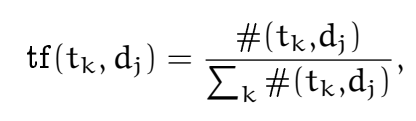
\includegraphics[scale=0.4]{images/lec07-pic10.png}
\end{figure}
где \#(tk,dj) - число, показывающее, сколько раз терм tk встречается в документе dj.
\end{frame}

\begin{frame}{Расстояние tf-idf}
\begin{block}{Обратная частота терма}
показывает, насколько терм вообще важен, насколько он характерен для данного массива текстов.
\end{block}
Чем реже встречается терм в имеющемся массиве, тем он характернее.
\begin{figure}[h]
\centering
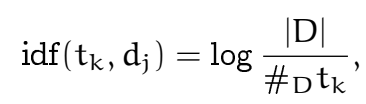
\includegraphics[scale=0.4]{images/lec07-pic11.png}
\end{figure}
где где D - имеющийся набор данных, а \#Dtk - количество документов из D, в которых хотя бы однажды встречается tk.
\end{frame}

\begin{frame}{Расстояние tf-idf}
Мера tdf для терма tk и документа dj в массиве D равна:
\begin{figure}[h]
\centering
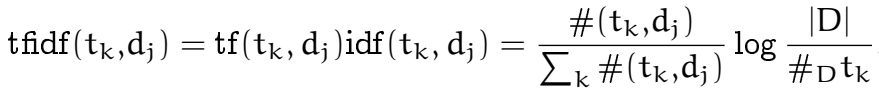
\includegraphics[scale=0.4]{images/lec07-pic12.png}
\end{figure}
Вектор весом можно нормализовать:
\begin{figure}[h]
\centering
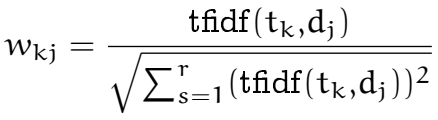
\includegraphics[scale=0.4]{images/lec07-pic13.png}
\end{figure}
Теперь документ можно представить в виде вектора, размерность которого равна количеству термов (важно сохранять словарь не слишком большим за счет удачного выбора термов).
\end{frame}

\begin{frame}{Расстояние между документами}
Расстояние между документами - используется не простое декартово расстояние, а угол между векторами, косинусоидальная мера похожести (cosine similarity measure):
\begin{figure}[h]
\centering
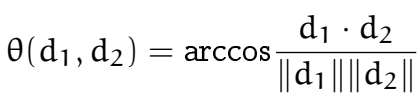
\includegraphics[scale=0.4]{images/lec07-pic14.png}
\end{figure}
\end{frame}